\section{系统测试}

\subsection{AquaTurnner 智能调参模块测试}

首先进行warm\_up得到一组参数和目标指标值的csv文件如图 \ref{test-turnner1} 所示,现在由于只调整AquaFS参数,参数空间较小,主要包括垃圾回收的gc相关参数,块大小以及zone的大小参数等,后续考虑在融合文件系统后加入inode相关参数。

\begin{figure}[htbp]
  \centering
  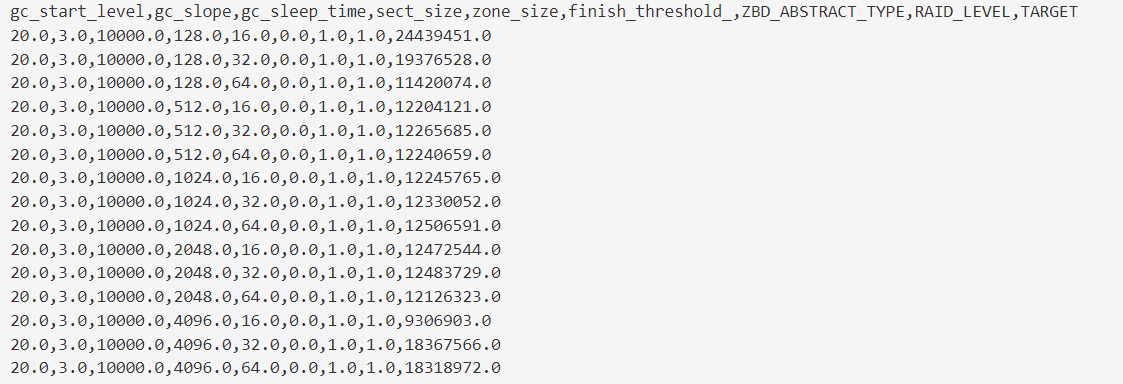
\includegraphics[width=0.85\textwidth]{fig/turnner1.png}
  \caption{ 调参测试数据 }
  \label{test-turnner1}
\end{figure}

设定参数进行AquaTuner的参数推荐流程,离散参数直接指定:

\begin{lstlisting}
SECT_SIZE_PARAM = 128
ZONE_SIZE_PARAM = 64
\end{lstlisting}

连续参数可以直接通过脚本defconfig获取。

接下来利用db\_bench进行参数跑分以及收集参数和目标值:

\begin{lstlisting}
  pre_throughput = 0
  now_throughput = 0
  for _ in range(1):
      sect_size = SECT_SIZE_PARAM
      zone_size = ZONE_SIZE_PARAM
      total_throughput = []
      for i in range(2):
          create_null_blk(sect_size, zone_size, 0, 64)
          os.system(CREATE_TMP_FILE)
          throughput_list = execute_adjust_param(2, sect_size, zone_size)
          total_throughput = total_throughput + throughput_list
          print("throughput list : {}".format(total_throughput))
          remove_null_blk()
      print("sect_size:{}".format(sect_size))
      print("zone_size:{}".format(zone_size))
      pre_throughput = now_throughput
      now_throughput = np.average(total_throughput)
\end{lstlisting}

代码的整体流程是,首先创建zone块,再在zone块上创建文件,得到跑分的吞吐量以及推荐参数,再将块zone块删除。

创建文件系统如下图所示,创建AquaFS的数据模块nullb0和作为log等文件存储的模块/tmp/aquafs。

\begin{lstlisting}
  CREATE_TMP_FILE = "mkdir -p /tmp/aquafs ;\
  sudo ../build/plugin/aquafs/aquafs mkfs --zbd nullb0 --aux-path /tmp/aquafs"
\end{lstlisting}

之后用db\_bench进行跑分,并进行智能调参模块的逻辑,按照指定推荐的离散参数跑一遍智能调参模块的结果如图 \ref{test-turnner2} 所示。

\begin{figure}[htbp]
  \centering
  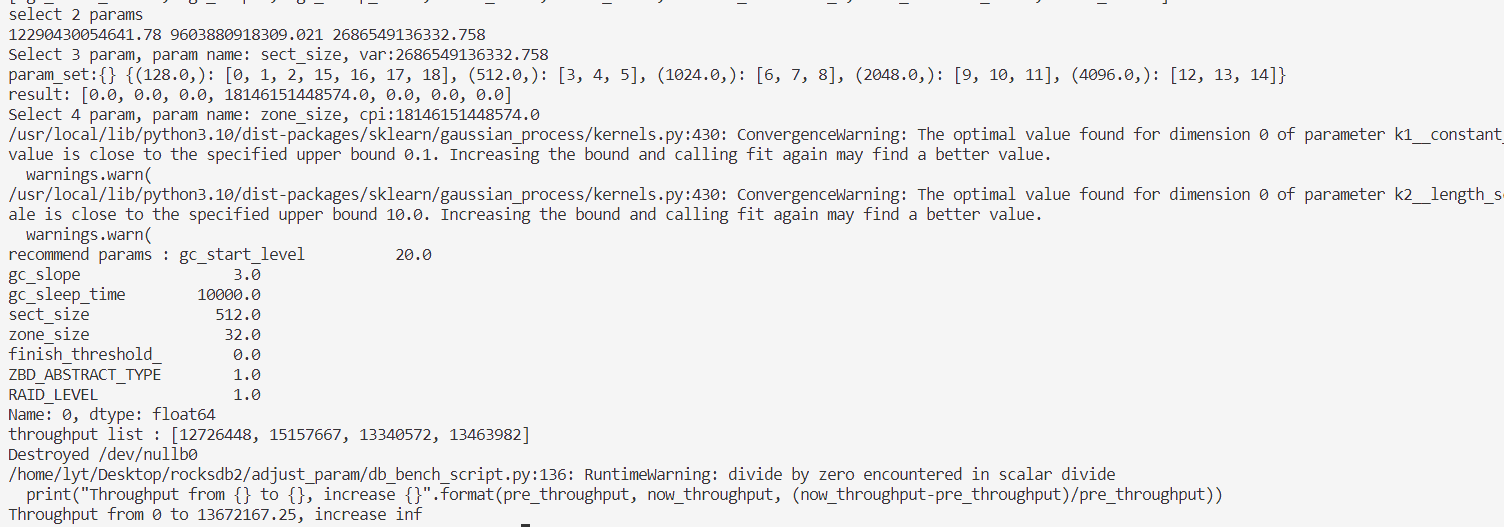
\includegraphics[width=0.85\textwidth]{fig/turnner2.png}
  \caption{ 调参测试过程 }
  \label{test-turnner2}
\end{figure}

在上图中推荐了两个参数,最重要的参数是sect\_size,其次是zone\_size,这符合现阶段的测试预期,因为我们的垃圾回收也就是gc还没有进行触发,,所以能够更改的参数现阶段只有块大小和zone\_size,而调参模块也根据现阶段的数据仓库中最优的参数进行了配置推荐。记录这里的平均吞吐量是13672167.25。

采用接下来的配置再进行测试:

\begin{lstlisting}
SECT_SIZE_PARAM = 512
ZONE_SIZE_PARAM = 32
\end{lstlisting}

最终结果如图 \ref{test-turnner3} 所示。

\begin{figure}[htbp]
  \centering
  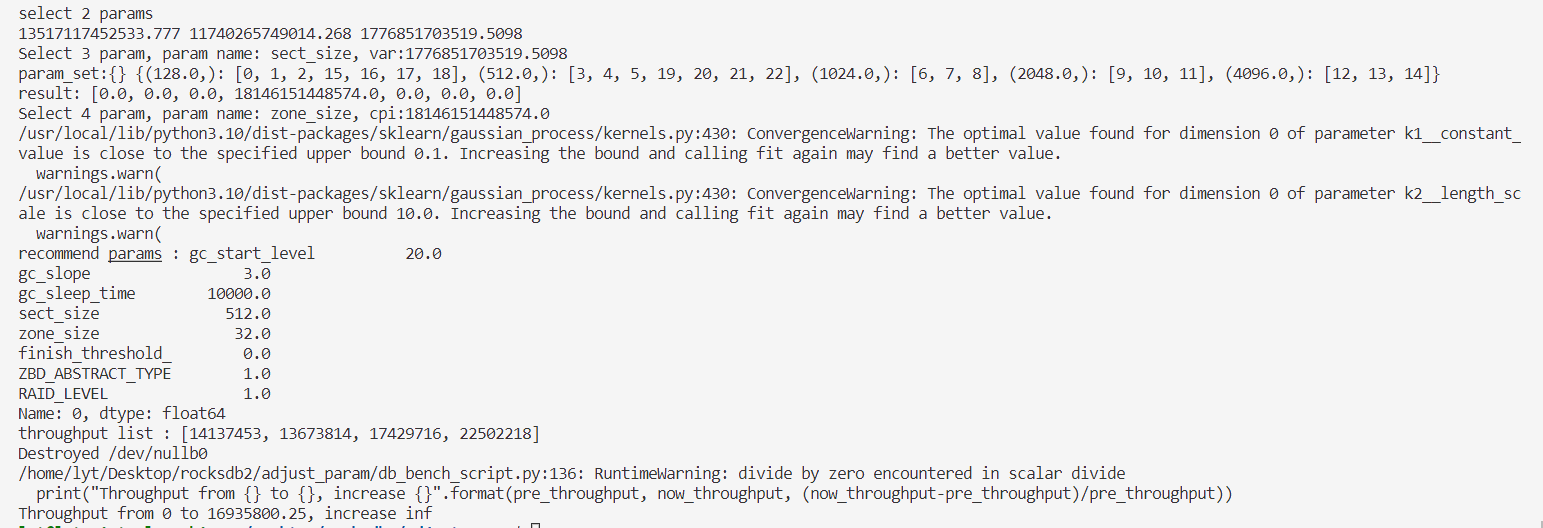
\includegraphics[width=0.85\textwidth]{fig/turnner3.png}
  \caption{ 调参测试结果 }
  \label{test-turnner3}
\end{figure}

平均吞吐量是16935800.25。相比于上一次的配置参数,吞吐量提升了23.87\%。

后续还将尝试测试触发gc来测试gc的参数,以及尝试融合文件系统后对整体的inode以及其他参数进行自动调整。

